\documentclass[fontset=none]{ctexart}

\setCJKmainfont{SimSun}
\setmonofont{DejaVu Sans Mono}
% Latin Modern

\setcounter{tocdepth}{5}
\setcounter{secnumdepth}{5}
% -1 part
% 0 chapter
% 1 section
% 2 subsection
% 3 subsubsection
% 4 paragraph
% 5 subparagraph

\usepackage{cite}
\usepackage{geometry}
\geometry{a4paper,scale=0.7}

\usepackage{algorithm}  
\usepackage{algorithmicx}  
\usepackage{algpseudocode}
\makeatletter
\newenvironment{breakablealgorithm}
  {% \begin{breakablealgorithm}
   \begin{center}
     \refstepcounter{algorithm}% New algorithm
     \hrule height.8pt depth0pt \kern2pt% \@fs@pre for \@fs@ruled
     \renewcommand{\caption}[2][\relax]{% Make a new \caption
       {\raggedright\textbf{\ALG@name~\thealgorithm} ##2\par}%
       \ifx\relax##1\relax % #1 is \relax
         \addcontentsline{loa}{algorithm}{\protect\numberline{\thealgorithm}##2}%
       \else % #1 is not \relax
         \addcontentsline{loa}{algorithm}{\protect\numberline{\thealgorithm}##1}%
       \fi
       \kern2pt\hrule\kern2pt
     }
  }{% \end{breakablealgorithm}
     \kern2pt\hrule\relax% \@fs@post for \@fs@ruled
   \end{center}
  }
\makeatother

\usepackage{amsmath}
\usepackage{amssymb}
\usepackage{graphicx}
\usepackage{subfigure}
\usepackage{changepage}
\usepackage{multirow}
\usepackage{url}

\usepackage{amsthm}
\newtheorem{theorem}{Theorem}[section]
\newtheorem{lemma}[theorem]{Lemma}
\newtheorem{proposition}[theorem]{Proposition}
\newtheorem{corollary}[theorem]{Corollary}
% \newtheorem{remark}{Remark}[section]
\newtheorem{example}{Example}[section]
\newenvironment{solution}{\begin{proof}[Solution]}{\end{proof}}
\theoremstyle{definition}
\newtheorem{definition}{Definition}[section]
\theoremstyle{remark}
\newtheorem*{remark}{Remark}

\usepackage[colorlinks, linkcolor=black, citecolor=blue, bookmarksnumbered]{hyperref}
% \hypersetup{
% 	colorlinks=true,
% 	linkcolor=cyan,
% 	filecolor=blue,      
% 	urlcolor=red,
% 	citecolor=green,
% }

\usepackage{fancyhdr}
\pagestyle{fancy}
\renewcommand{\sectionmark}[1]{\markright{\thesection\ #1}}
\fancyhf{}
\cfoot{\thepage}
\lhead{\rightmark}
% \rightmark 当前的节名
% \leftmark 当前的章名
% \(l/c/r)head{}, \(l/c/r)foot{}
\renewcommand{\headrulewidth}{0.4pt}
\renewcommand{\footrulewidth}{0pt}

\renewcommand\refname{References}
\renewcommand\contentsname{Content}
\renewcommand\figurename{Figure}

\begin{document}

\begin{titlepage}
    \begin{center}
        \vspace*{1cm}
            
        \Huge
        \textbf{Traffic Predicion With Advanced Graph Neural Networks}
            
        \vspace{0.5cm}
        \LARGE
        End-term Report\\
            
        \vspace{1.5cm}
            
        \textbf{11812804}  董\quad 正\\
        \textbf{11813225}  王宇辰\\
        \textbf{11811305}  崔俞崧\\

        \vspace{0.5cm}
        Supervisior: 宋轩
            
        \vfill
            
        
\includegraphics[width=\textwidth]{images/sustc.png}
            
        \vspace{0.2cm}
            
        \Large
        Department of Computer Science and Engineering\\
        \vspace{0.5cm}
        Jan. 2021
            
    \end{center}
\end{titlepage}

\tableofcontents

\clearpage
\section{Preliminaries}
\subsection{Review}
\subsubsection{TTE}
\textbf{Travel Time Estimation (TTE)} is one of the most important researching topic in the traffic forecasting field. 
Estimating the travel time of any path in a city is of great importance to traffic monitoring, route planning, ridesharing, taxi dispatching, etc.
On Sep. 2020, DeepMind published a blog named \textit{Traffic prediction with advanced Graph Neural Networks}. 
This blog briefly described the whole industrial structure of estimated times of arrival (ETAs) techniques applied in Google Map but did not given any detailed implementation or any code.
Our work is based on the model structure of TTE proposed in the blog.
\begin{figure}[htb]
    \centering
    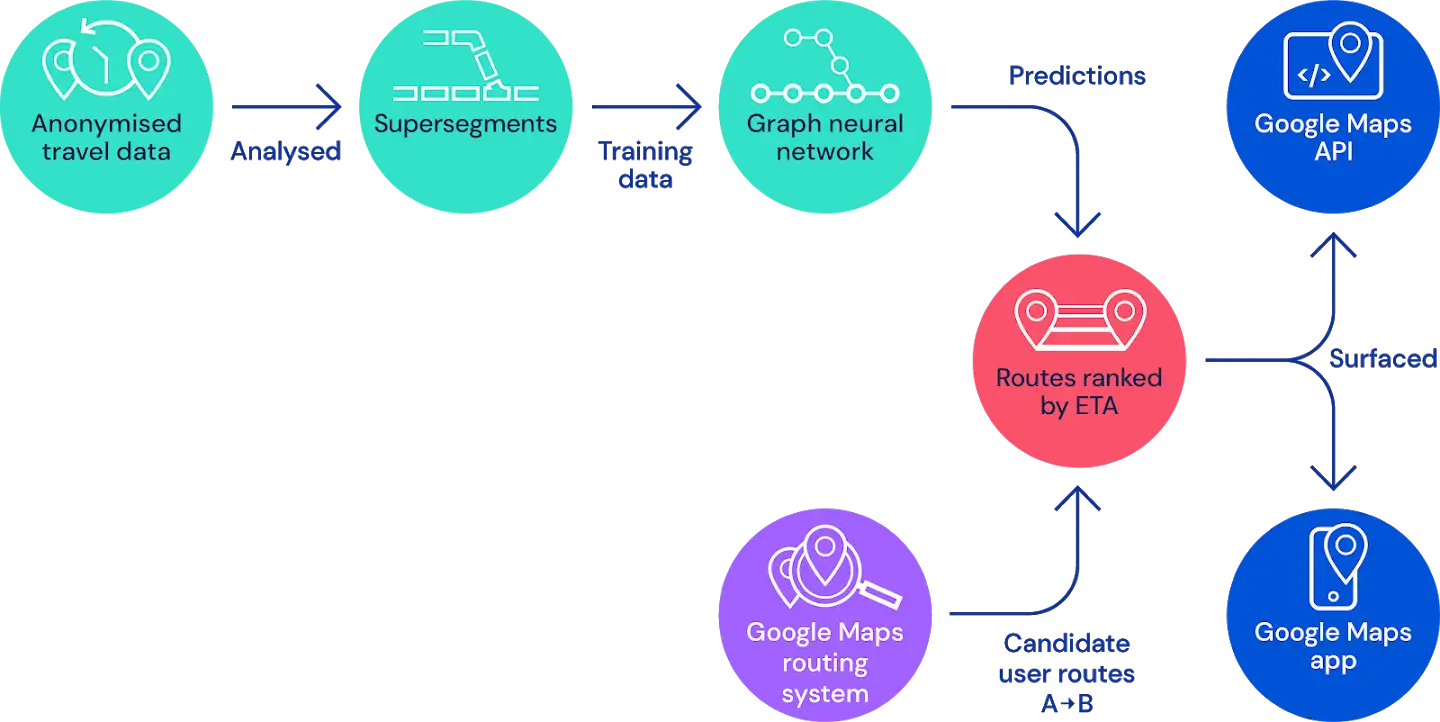
\includegraphics[width=0.9\textwidth]{images/architecture.png}
    \caption{Architecture}
    \label{fig1}
\end{figure}

\subsubsection{Goal}
Our ultimate goal (tentative) is to implement the industrial structure and apply it to the open source databases in China, then compare the performance with the state-of-the-art structures and find its application value.
This semester, we will first learn about the relative algorithms. More specifically, the two main algorithm we will use: TTE algorithm and Graph Neural Network (GNN). After that, we will learn the methods of processing traffic data. Finally, we combine the algorithms and apply them on some open source database.

\subsection{Introduction}
In the last stage, we have got some open source data and learned how to process the
data. And we got deep in the code of \textit{DeepTTE} and researched on a new concept
called \textbf{Travel Time Index (TTI)}. In addition, we proposed a new computing process of \textit{Supersegment}.

Breifly, we will state our work in this report as:
\begin{itemize}
    \item DeepTTE Result Analysis by 王宇辰
    \item Calculation of TTI by 崔俞崧
    \item An implementation of Supersegment by 董正
\end{itemize}

\clearpage
\section{DeepTTE Result Analysis}

    Due to previous result on training loss, although training loss is level off to 0, test loss remians about 0.2, as shown in figure \ref{head}. I tried to change the hyperparameters, but cannot get an explicit better result. Then, a deep research on the result is applied.

    \begin{figure}[H]
        \centering
        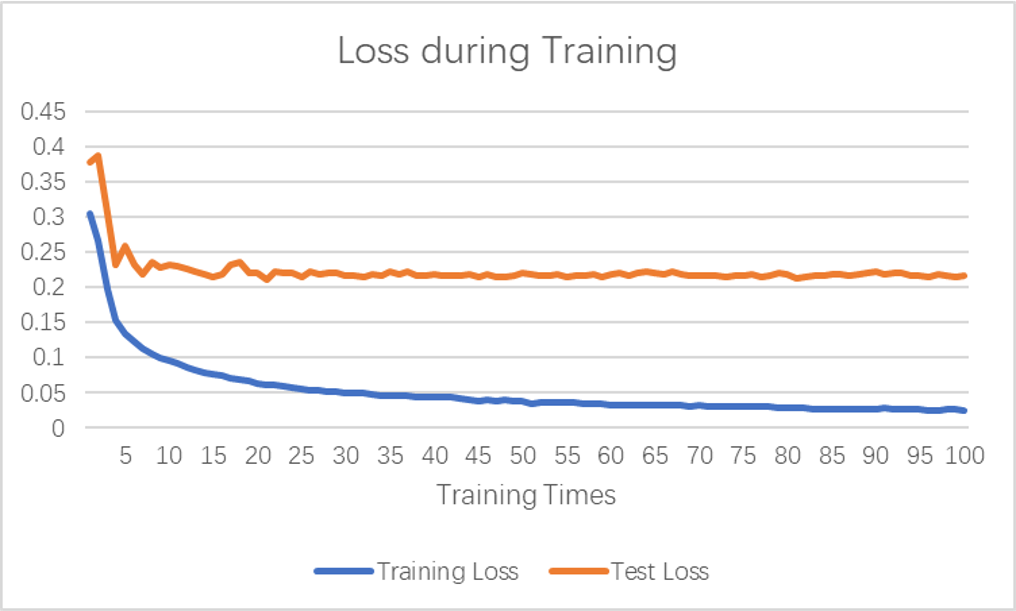
\includegraphics[width=0.8\textwidth]{src/Head.png}
        \newline
        \label{head}
        \caption{Total Loss during Training}
    \end{figure}

        \subsection{The training process}

            As shown in figure \ref{Training}, the training result is shown every 20 epoches. We can simply analyze by using $\frac{Predict\ Time}{Exact\ Time}$ to find the trend during training.

            In the first epoch, shown in figure \ref{Training1}, the average ratio is 0.5, with great difference from 1.0.

            In the 20th epoch, shown in figure \ref{Training2}, the average ratio is 0.8, with distributed ratio.

            In the 40th epoch, shown in figure \ref{Training3}, the average ratio is around 0.8 - 0.9, with ratio < 0.8 reduced and retio > 0.8 increased.

            In the 60th epoch, shown in figure \ref{Training4}, the average ratio is 0.8, with ratio < 0.8 less than 0.2.

            In the 80th epoch, shown in figure \ref{Training5}, the average ratio is around 0.8 - 0.9, with ratio > 0.9 reduced.

            In the 100th epoch, shown in figure \ref{Training6}, the average ratio is 0.8, with gradually form an exponential function distribution.

            \begin{figure}[H]
                \centering
                \subfigure[Epoch 1]{
                    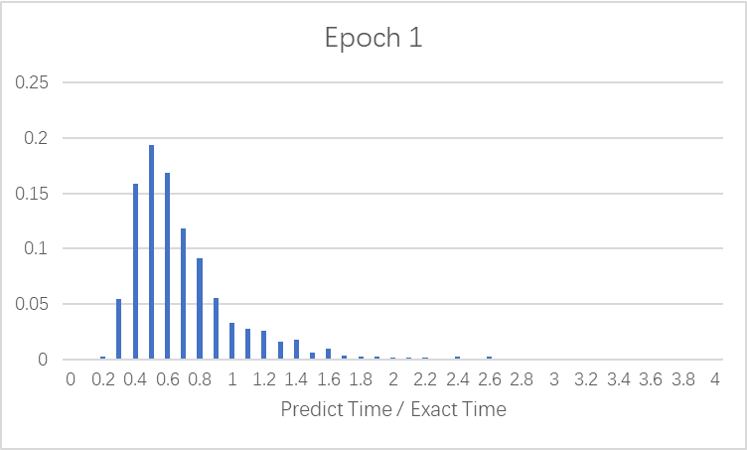
\includegraphics[width=0.4\textwidth]{src/Training1.png}
                    \label{Training1}
                }
                \quad
                \subfigure[Epoch 20]{
                    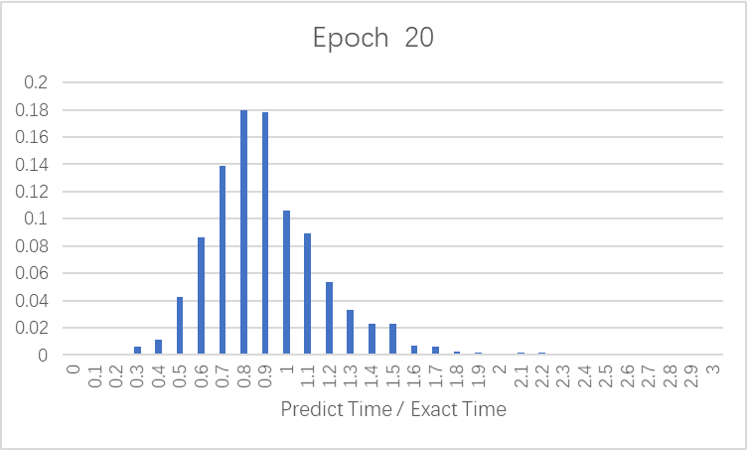
\includegraphics[width=0.4\textwidth]{src/Training2.png}
                    \label{Training2}
                }
                \newline
                \subfigure[Epoch 40]{
                    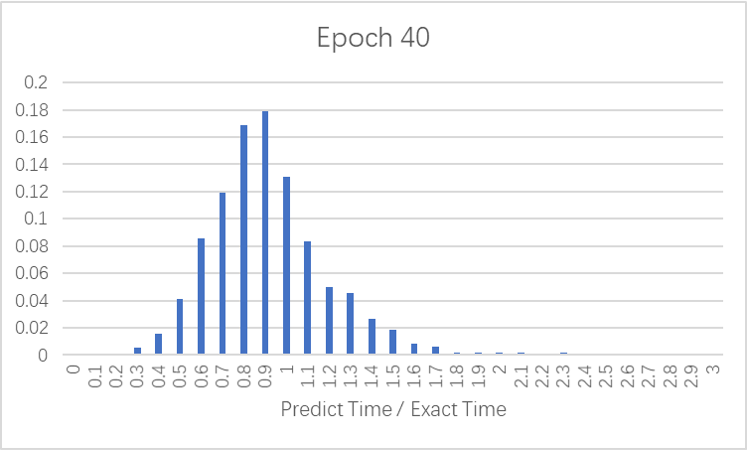
\includegraphics[width=0.4\textwidth]{src/Training3.png}
                    \label{Training3}
                }
                \quad
                \subfigure[Epoch 60]{
                    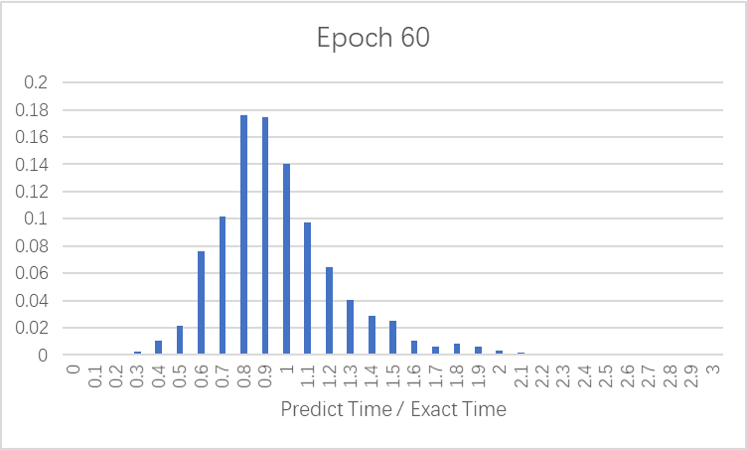
\includegraphics[width=0.4\textwidth]{src/Training4.png}
                    \label{Training4}
                }
                \newline
                \subfigure[Epoch 80]{
                    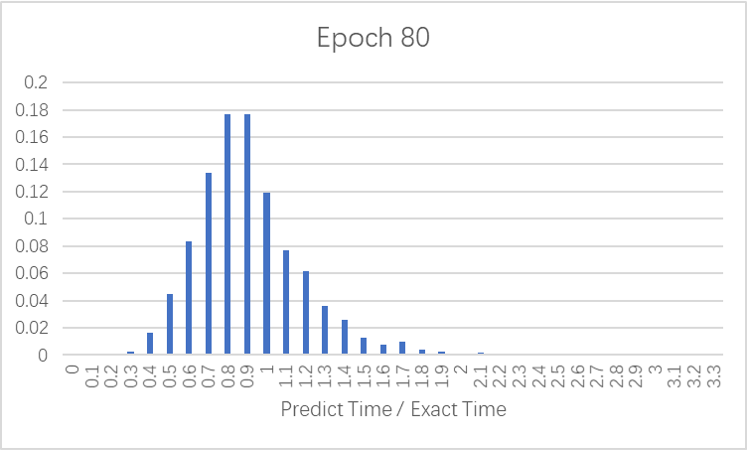
\includegraphics[width=0.4\textwidth]{src/Training5.png}
                    \label{Training5}
                }
                \quad
                \subfigure[Epoch 100]{
                    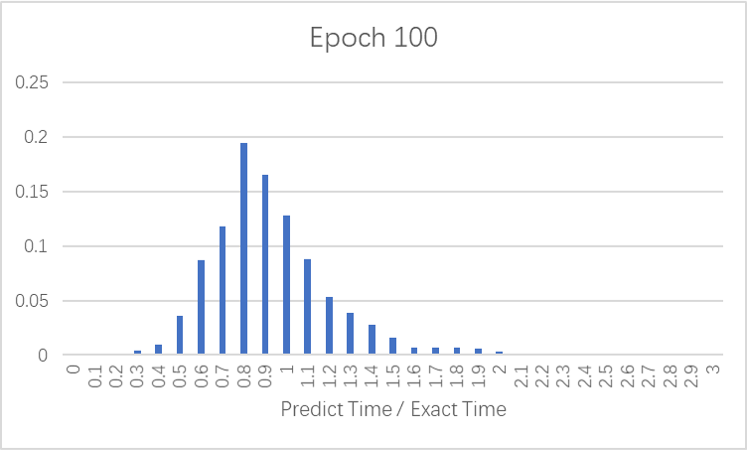
\includegraphics[width=0.4\textwidth]{src/Training6.png}
                    \label{Training6}
                }
                \newline
                \caption{Total Loss during Training}
                \label{Training}
            \end{figure}

        \subsection{The Exact Time}

            The exact time distribution is shown in figure \ref{Distribution}, mainly within 480s - 2400s, about 8min - 40min. Thus, we choose to analyze every 10min, equal to 600s.

            \begin{figure}[H]
                \centering
                \subfigure[In number]{
                    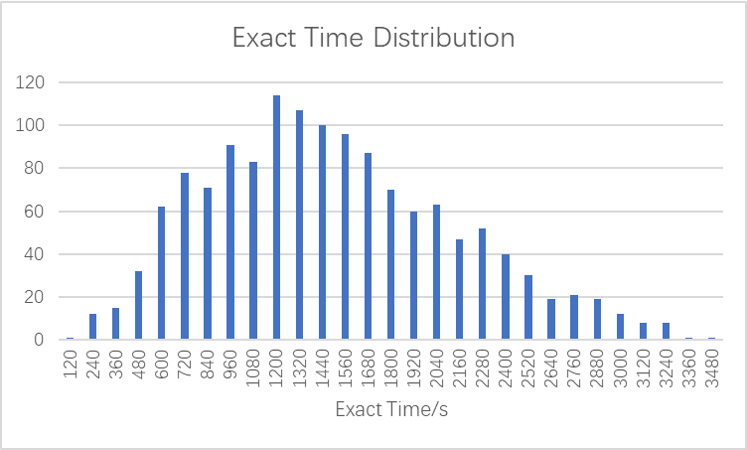
\includegraphics[width=0.4\textwidth]{src/Distribution1.png}
                }
                \quad
                \subfigure[In probability]{
                    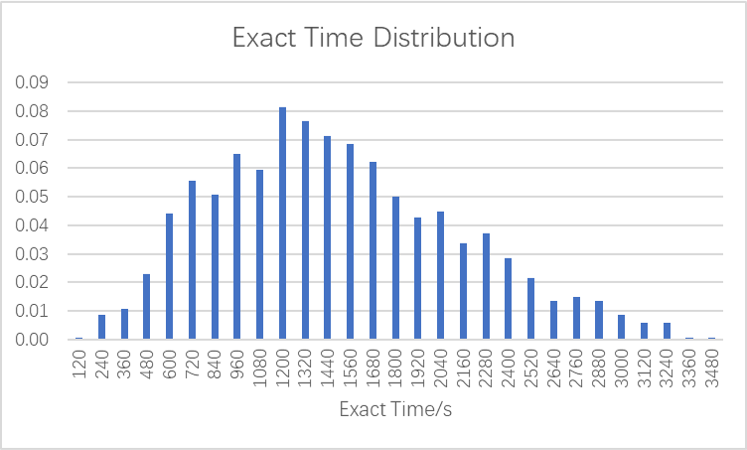
\includegraphics[width=0.4\textwidth]{src/Distribution2.png}
                }
                \newline
                \caption{Exact Time Distribution}
                \label{Distribution}
            \end{figure}

            Around 600s, as shown in figure \ref{Exact1}, Ratio is higher than 1.0, prediction is about 30\% over exact time.

            Around 1200s, as shown in figure \ref{Exact2}, Ratio is about 0.9 - 1.0, prediction is most accurate around 1200s.

            Around 1800s, as shown in figure \ref{Exact3}, Ratio is around 0.9, prediction is about 10\% below exact time, can be applied at all.

            Around 2400s, as shown in figure \ref{Exact4}, Ratio is about 0.6 - 0.9, prediction is inaccurate as it is about 30\% difference in average.

            \begin{figure}[H]
                \centering
                \subfigure[Around 600s]{
                    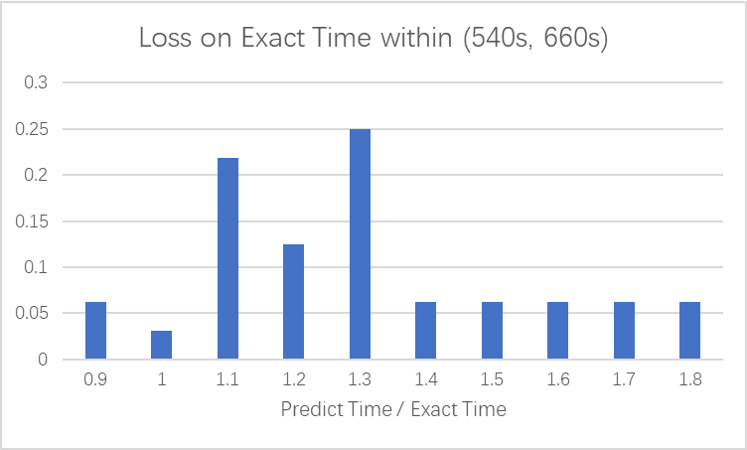
\includegraphics[width=0.4\textwidth]{src/Exact1.png}
                    \label{Exact1}
                }
                \quad
                \subfigure[Around 1200s]{
                    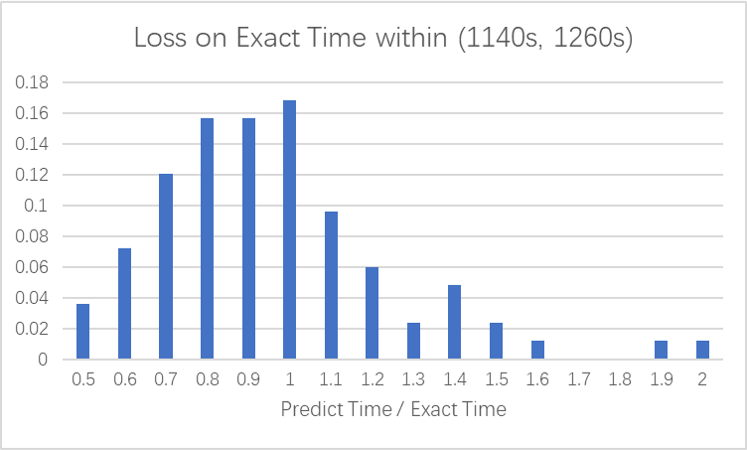
\includegraphics[width=0.4\textwidth]{src/Exact2.png}
                    \label{Exact2}
                }
                \newline
                \subfigure[Around 1800s]{
                    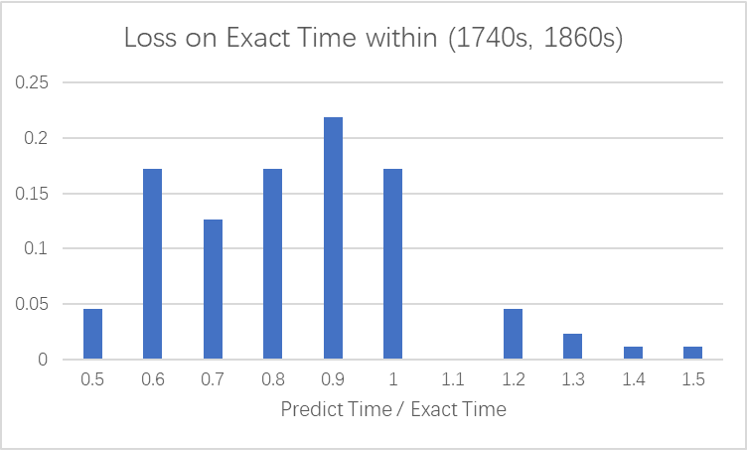
\includegraphics[width=0.4\textwidth]{src/Exact3.png}
                    \label{Exact3}
                }
                \quad
                \subfigure[Around 2400s]{
                    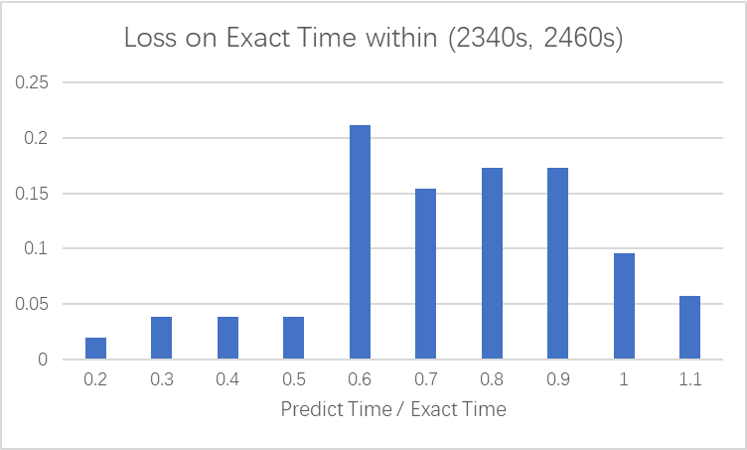
\includegraphics[width=0.4\textwidth]{src/Exact4.png}
                    \label{Exact4}
                }
                \newline
                \caption{Sample Distribution}
                \label{Samples}
            \end{figure}

        \subsection{Conclusion}

            Return to the question from figure \ref{head}, we can find out something.

            \begin{itemize}

                \item In the training process, the ratio is gradually centerlized to 0.8 - 1.0.
                
                \item Predict time around 1200s – 1800s is accurate, about 10\% error. 
            
            \end{itemize}

\clearpage
\section{Travel Time Index}
The TTI (Travel Time Index) industry's most used evaluation index of urban congestion degree is the ratio of the actual travel time and the free flow time.
\begin{equation}
  TTI=\frac{\sum_{i=1}^N\frac{L_i}{V_i}\cdot W_i}{\sum_{i=1}^N\frac{L_i}{V_{free\_i}}\cdot W_i} \notag
\end{equation}
\begin{itemize}
  \item $L_i$: length of the road
  \item $W_i$: weight of road
  \item $V_i$: real time traffic information
  \item $V_{free\_i}$: free flow velocity
\end{itemize}

\subsection{Dataset}
\begin{itemize}
    \item Data source: Didi Chuxing GAIA Intiative
    \item Region: Chengdu
    \item Time: 2018-10-01 to 2018-12-01
    \item Content:
        \begin{itemize}
            \item GPS track of taxis with timestamps
            \item Coordinate of road and district boundaries
            \item TTI and average speed of districts
        \end{itemize}
\end{itemize}

\clearpage
\subsection{Computing TTI}
To calculate the TTI, the most important thing is to calculate the average speed of the section and the free flow speed. In order to get the average speed of the road section, it is necessary to calculate through a large number of track data.
First, select the section of road to be calculated and the time (here we take the north of the first ring road.;10:00 a.m.-10:10 a.m. as an example), and draw all the tracks and sections as shown in the figure below. Note that in order to make the trajectories clearly visible, 20 trajectories are selected here for drawing demonstration. The number of trajectories in the actual calculation process is far greater than that shown in the figure.
(The black line segment represents the vehicle track and the red line segment represents the road)
\begin{figure}[htb]
  \centering
  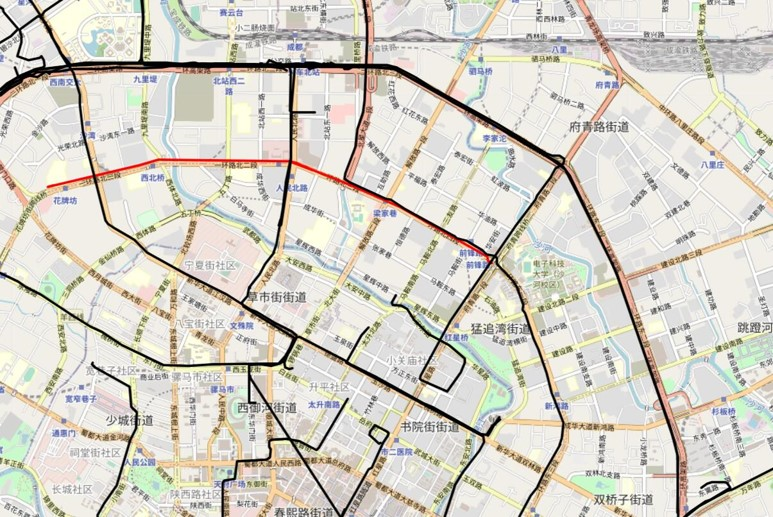
\includegraphics[width=\textwidth]{images/tti3-1.jpg}
\end{figure}

\clearpage
Then, the track is matched with the section. The unmatched track is removed, and only the successfully matched track is retained. The matching method is mainly carried out by judging the distance between the track point and the road section. Therefore, even if the track only intersects with the road section, it will be successfully matched here.
\begin{figure}[htb]
  \centering
  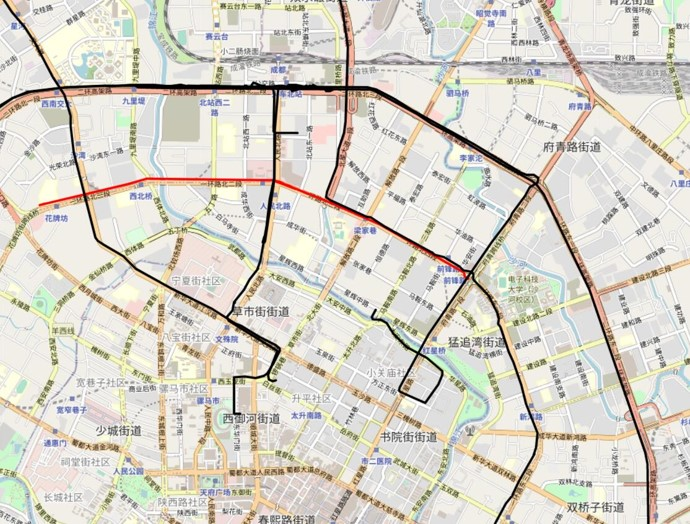
\includegraphics[width=\textwidth]{images/tti3-2.jpg}
\end{figure}

\clearpage
However, a track that intersects rather than overlaps with a section of road is considered a match, but this type of track does not reflect the traffic situation of the section at all.
Therefore, the overlap between the successfully matched track and the road section is then calculated. If the overlap is too small, the track will be deleted to ensure that the successfully matched track is all the track that has been traveled in the road section.
\begin{figure}[htb]
  \centering
  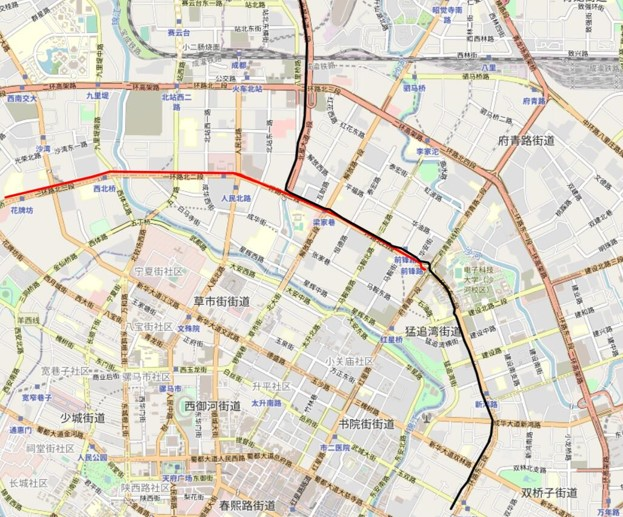
\includegraphics[width=\textwidth]{images/tti3-3.jpg}
\end{figure}

After data processing, the average speed of the section is calculated.
Firstly, the processed track is used to calculate the average velocity of the track, which is set as $V_t$ ($t$ represents the number of tracks).
After the average velocity of each track is obtained, the average velocity $V_{avg}$ of this section is calculated as followed: (Here $n$ represents the total number of matched sections)
\begin{equation}
  v_{avg}=\frac 1n\sum_{t=1}^n v_t \notag
\end{equation}

Secondly, the free flow velocity of the section is calculated.
The speed between 4:00 and 4:30 is selected here as the free flow speed.

\subsection{Result}
\begin{figure}[htb]
  \centering
  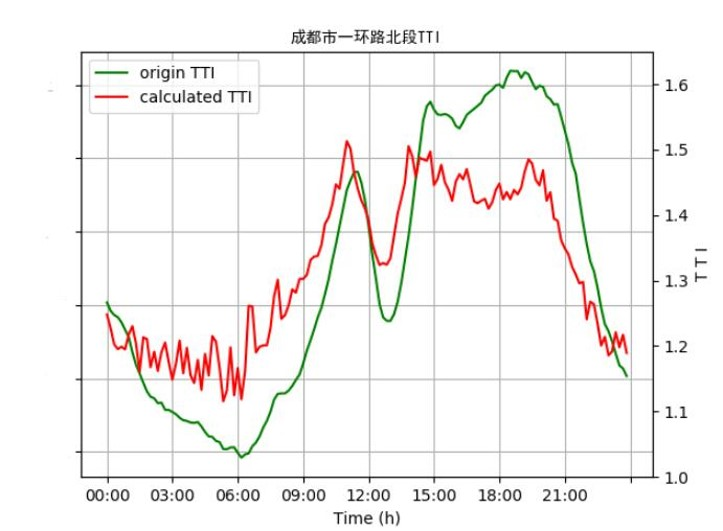
\includegraphics[width=\textwidth]{images/tti3-4.jpg}
\end{figure}

There is a big difference between the calculated TTI and the reference TTI. The most likely reason is that the average speed of the road section used in the calculation is quite different from the official calculation method.

\clearpage
To improve it:

First, when calculating the average speed of a section, the track is no longer the whole track, but only the track that overlaps with the section is used to calculate the speed.
\begin{figure}[htb]
  \centering
  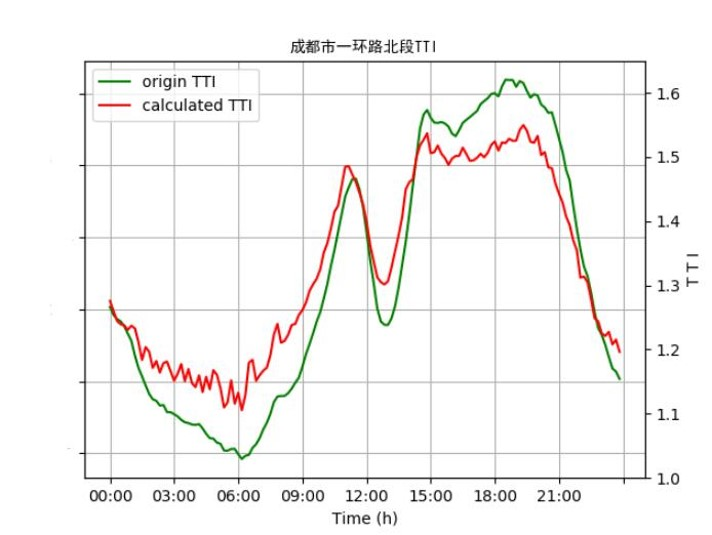
\includegraphics[width=\textwidth]{images/tti3-5.jpg}
\end{figure}

\clearpage
Secondly, considering that the traffic on the road is two-way, and there has no relationship between two directions of traffic flow. When calculating the trajectory velocity, further screening is carried out to select only trajectories in the same direction.
\begin{figure}[htb]
  \centering
  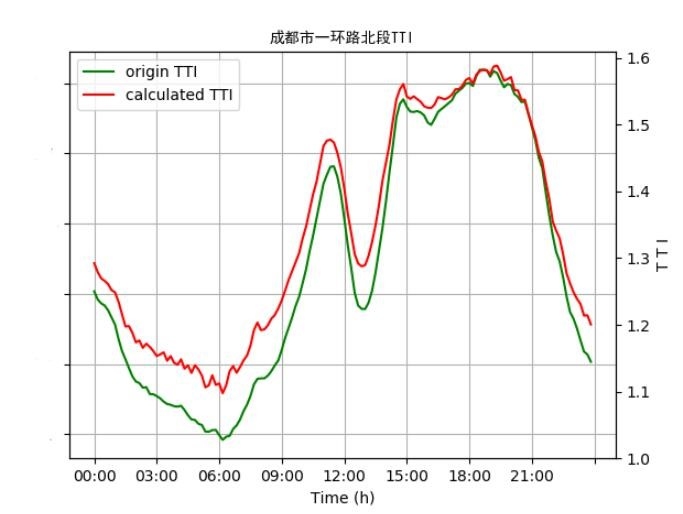
\includegraphics[width=\textwidth]{images/tti3-6.jpg}
\end{figure}

\subsection{Error Analysis}
Although the calculation model of TTI has been improved, there are still some errors between the obtained results and the official reference values.
Possible reasons are as follows:
\begin{enumerate}
  \item The official TTI calculation adopts the speed of all vehicles, but I only have the trajectory data of taxis while do the calculation.
  \item The official may obtain the vehicle speed through the speed camera sampling in multiple areas of a road, and the way to obtain the vehicle speed is quite different.
  \item There is no standard answer to the selection of free flow speed. Here, different values may be selected as the free flow speed. And the results can be quite different.
\end{enumerate}

\clearpage
\section{Implementation of Supersegment}
\subsection{Dataset}
\begin{itemize}
    \item Data source: Didi Chuxing GAIA Intiative
    \item Region: Chengdu
    \item Time: 2018-10-01 to 2018-12-01
    \item Content:
        \begin{itemize}
            \item GPS track of taxis with timestamps
            \item Coordinate of road and district boundaries
            \item TTI and average speed of districts
        \end{itemize}
\end{itemize}
\begin{figure}[htb]
  \centering
  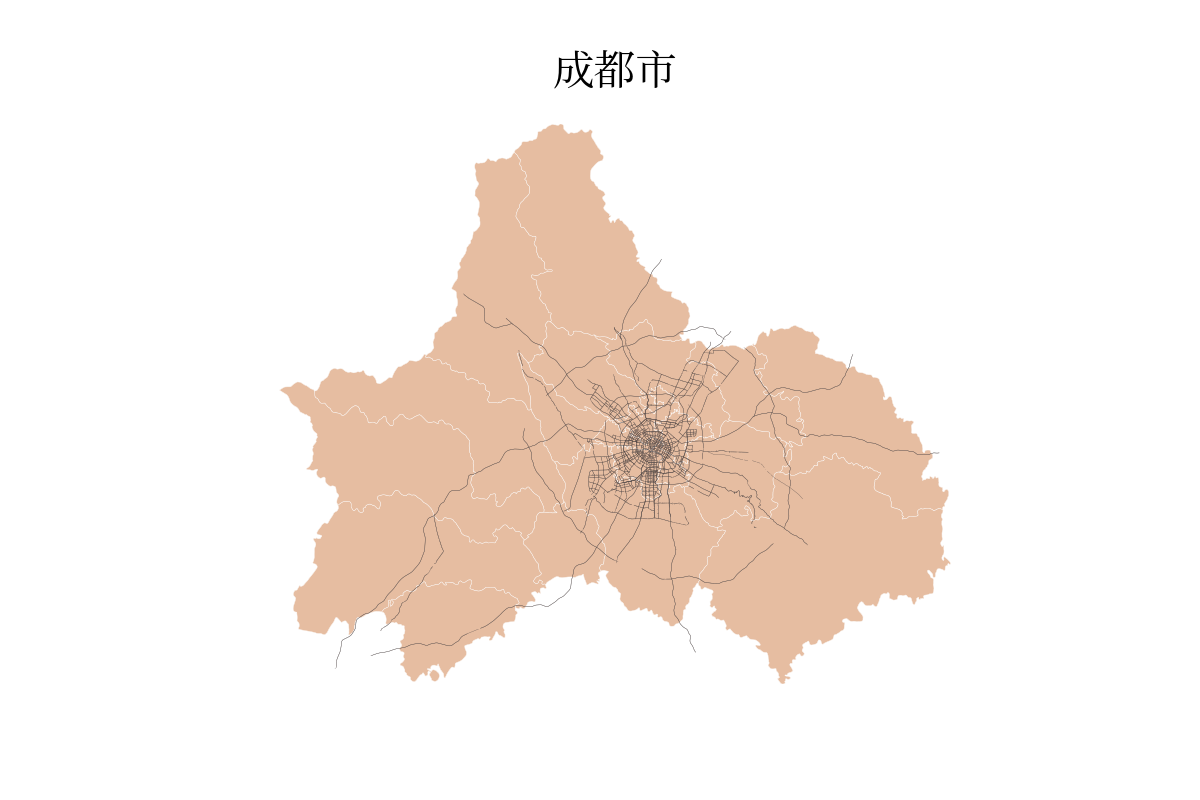
\includegraphics[width=\textwidth]{images/成都市.png}
  \caption{Cheng Du}
  \label{fig: chengdu}
\end{figure}

\subsection{Model Design}
In this section, I will propose a model to compute Supersegments.
At the very first, I need to ensure that I will base on \textbf{speed} to do the division.
There is a three-step approach of my design:
\begin{enumerate}
    \item Locate GPS coordinates of taxis into corresponding roads
    \item Use the timestamps to calculate average speed and regead it as the instantaneous speed of midpoint
    \item Apply clustering algorithm to these midpoints
\end{enumerate}

First, since we know the boundaries of the roads, we can determine the coordinate is on which road.
After that, we draw the GPS points on the road. Because we know the timestamp of each point, we can 
calculate the average speed of two adjacent points and just consider it as the speed of their midpoint.
Note that the closer the points are, the closer the average speed is to the actual instantaneous speed.
So the best way is to select adjacent points if our data is abundant.
\begin{figure}[htb]
  \centering
  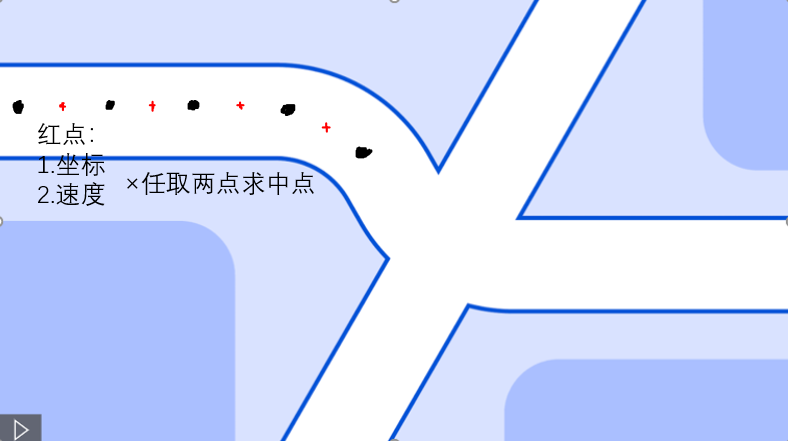
\includegraphics[width=0.9\textwidth]{images/midpoints.png}
  \caption{Find the midpoints}
  \label{fig: midpoint}
\end{figure}

Next step is to apply clustering algorithm like \textit{K-Means} to find a certain number of clusters
of the midpoints.
Every midpoint has three features:
\begin{itemize}
  \item longitude
  \item latitude
  \item speed
\end{itemize}

So actually this is a three-dimension clustering, but the result we need is two-dimensional, which means
we need to balance the weight of these features carefully to get a correct partition.
And finally, these clusters give us segments.
\begin{figure}[h]
  \centering
  \subfigure[Clusters] {
    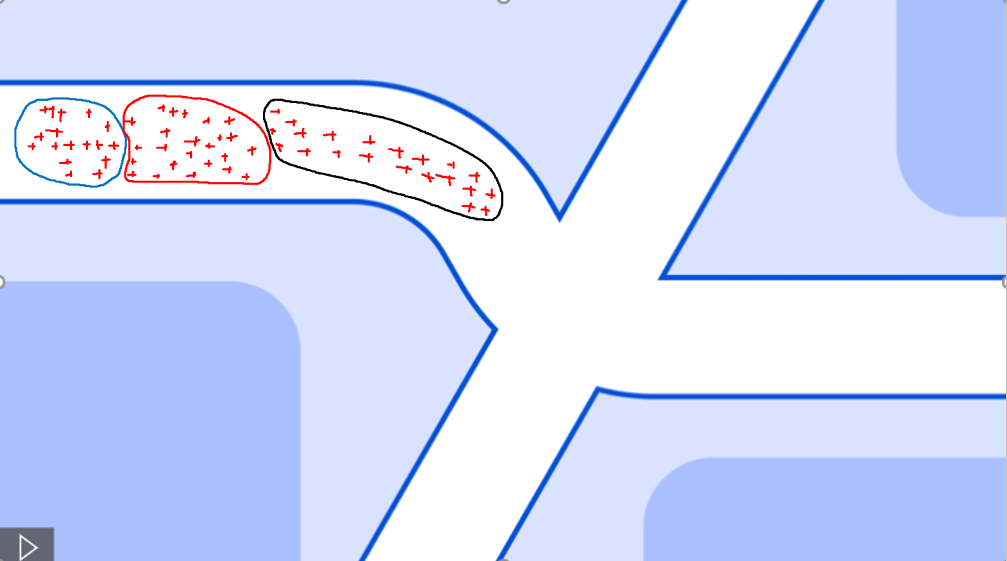
\includegraphics[width=0.45\textwidth]{images/cluster.png}
  }
  \quad
  \subfigure[K-Means Example] {
    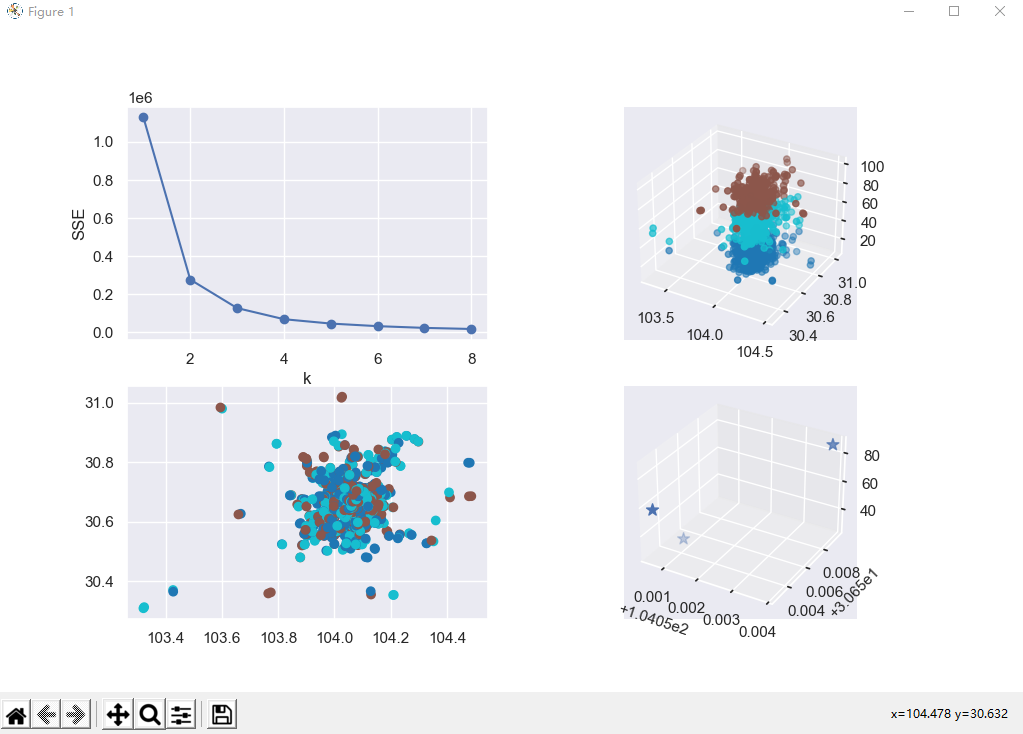
\includegraphics[width=0.45\textwidth]{images/kmeans.png}
  }
\end{figure}

\clearpage
\subsection{Implementation}
Firstly, we show the tracks of taxis on the map:
\begin{figure}[htb]
  \centering
  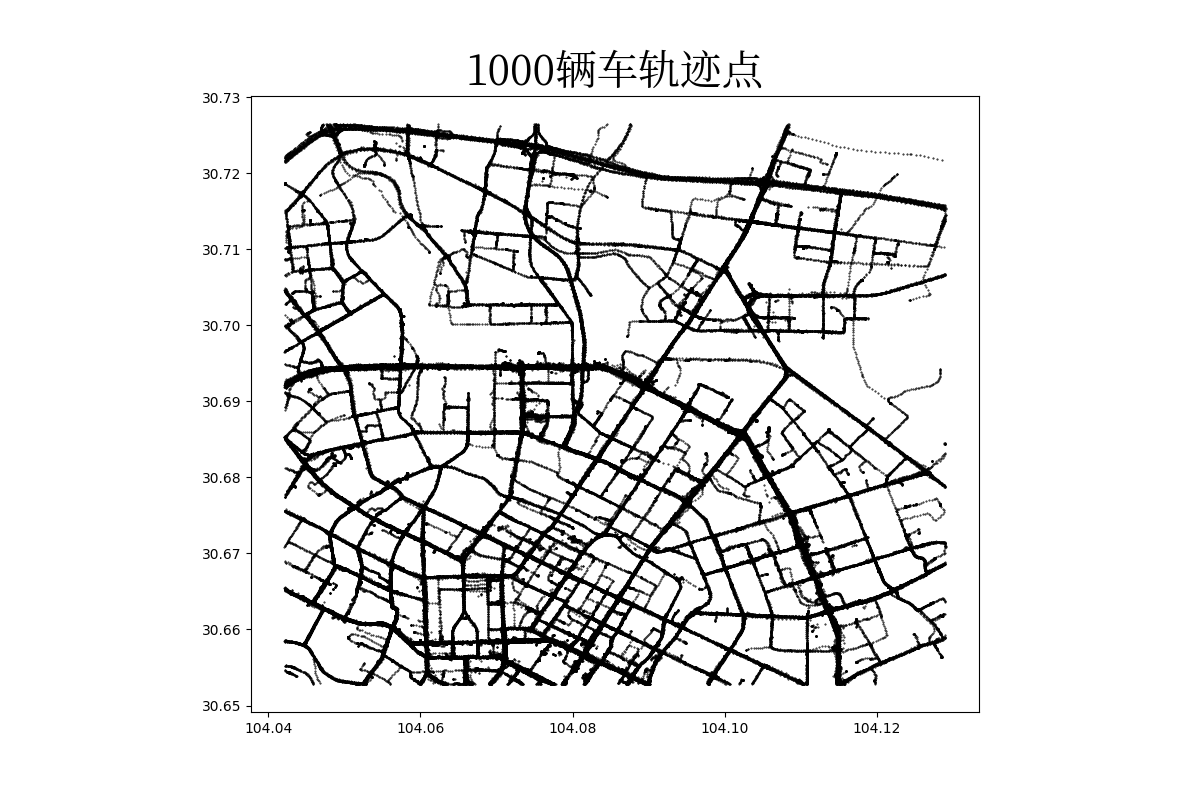
\includegraphics[width=\textwidth]{images/1000辆车轨迹点.png}
  \caption{Tracks}
  \label{fig: tracks}
\end{figure}

For convenience, we choose a road at the left bottom corner, which is almost horizontal.

The range of the road is about $(104.06060, 30.66680)$ to $(104.07049, 30.66718)$.
Then screen out the points.
\begin{figure}[htb]
  \centering
  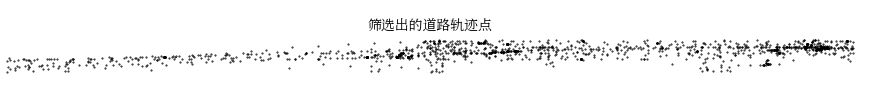
\includegraphics[width=\textwidth]{images/temp.png}
  \caption{Points}
  \label{fig: points}
\end{figure}

After that, we calculate the coordinate and speed of midpoints.
Note that there is no need to compute the actual speed, so the fomula is given below:
\begin{equation}
  v=\frac{\sqrt{(x_1-x_2)^2+(y_1-y_2)^2}}{t}
  \notag
\end{equation}
where $x$ is longitude, $y$ is latitude and $t=10s$ is given by the dataset.
\begin{figure}[htb]
  \centering
  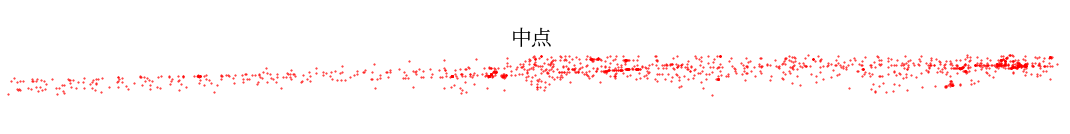
\includegraphics[width=\textwidth]{images/1000辆车中点.png}
  \caption{Midpoints}
  \label{fig: Midpoints}
\end{figure}

Then apply \textit{K-Means} algorithm on the midpoints.

Using 5000 taxis' data, and determine the value of $k$ is $4$.
\begin{figure}[htb]
  \centering
  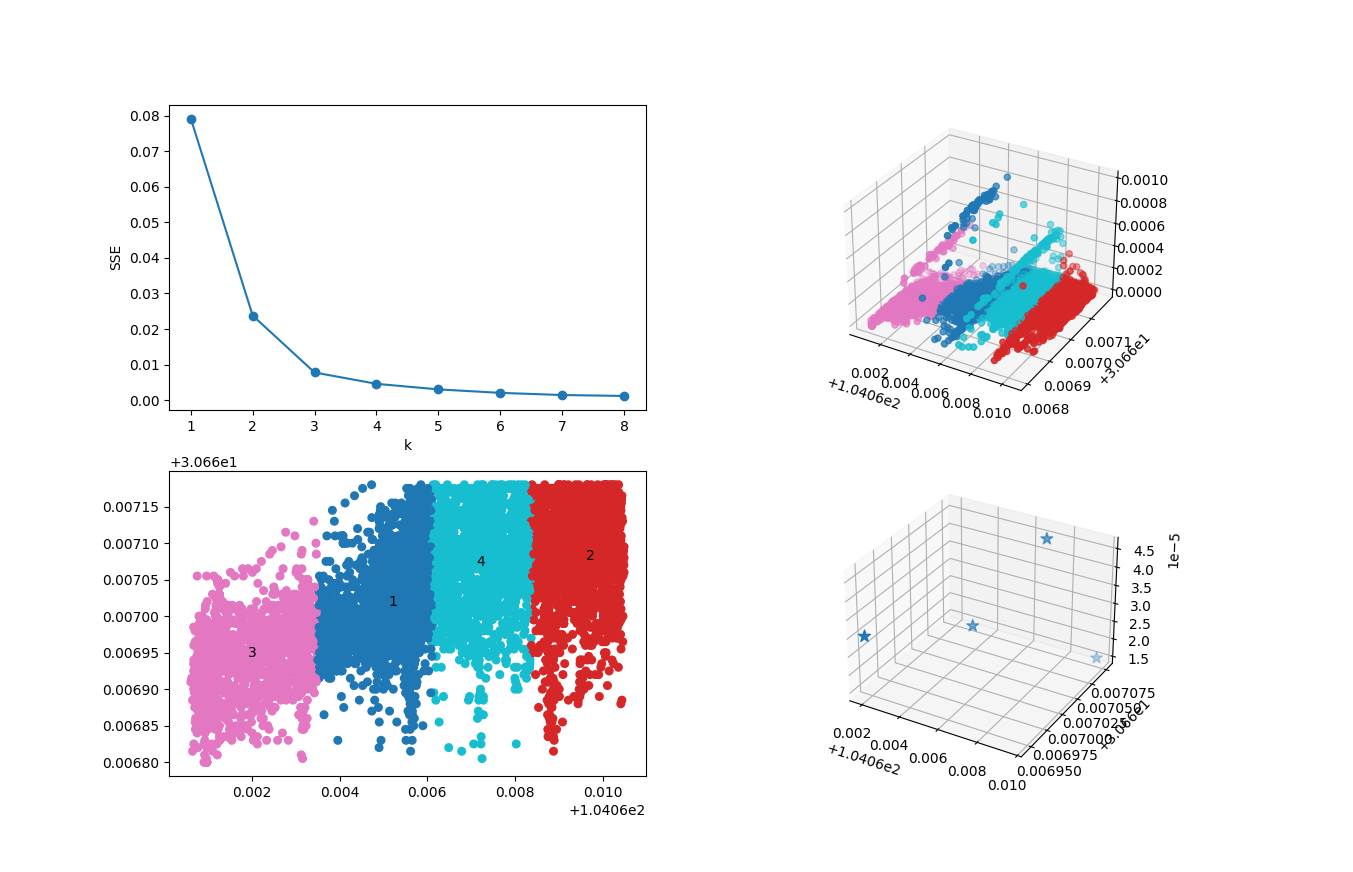
\includegraphics[width=\textwidth]{images/5000辆车kmeans.png}
  \caption{K-Means}
  \label{fig: 5000}
\end{figure}

\clearpage
Using 10000 taxis' data:
\begin{figure}[htb]
  \centering
  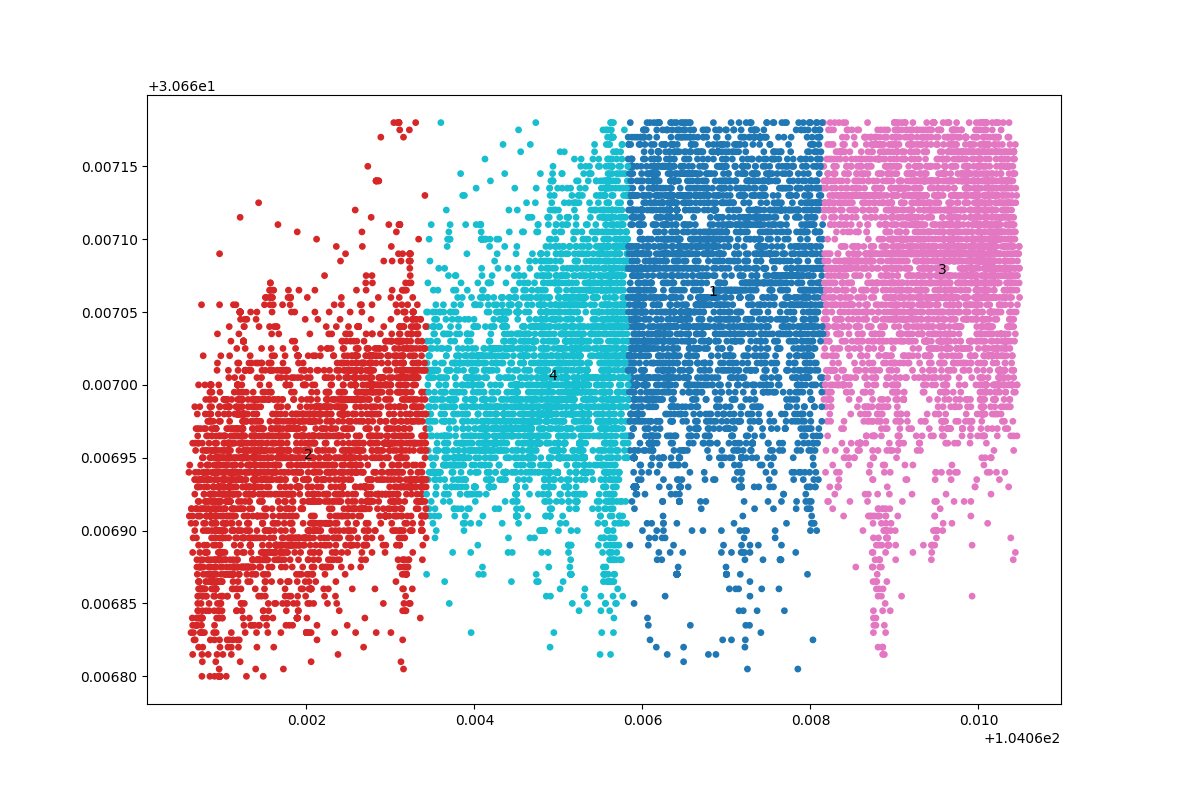
\includegraphics[width=\textwidth]{images/10000辆车kmeans.png}
  \caption{10000 Taxis K-Means}
  \label{fig: 10000}
\end{figure}

We already have a fairly acceptable result, but still can be more accurate.

\clearpage
Using 20000 taxis' data:
\begin{figure}[htb]
  \centering
  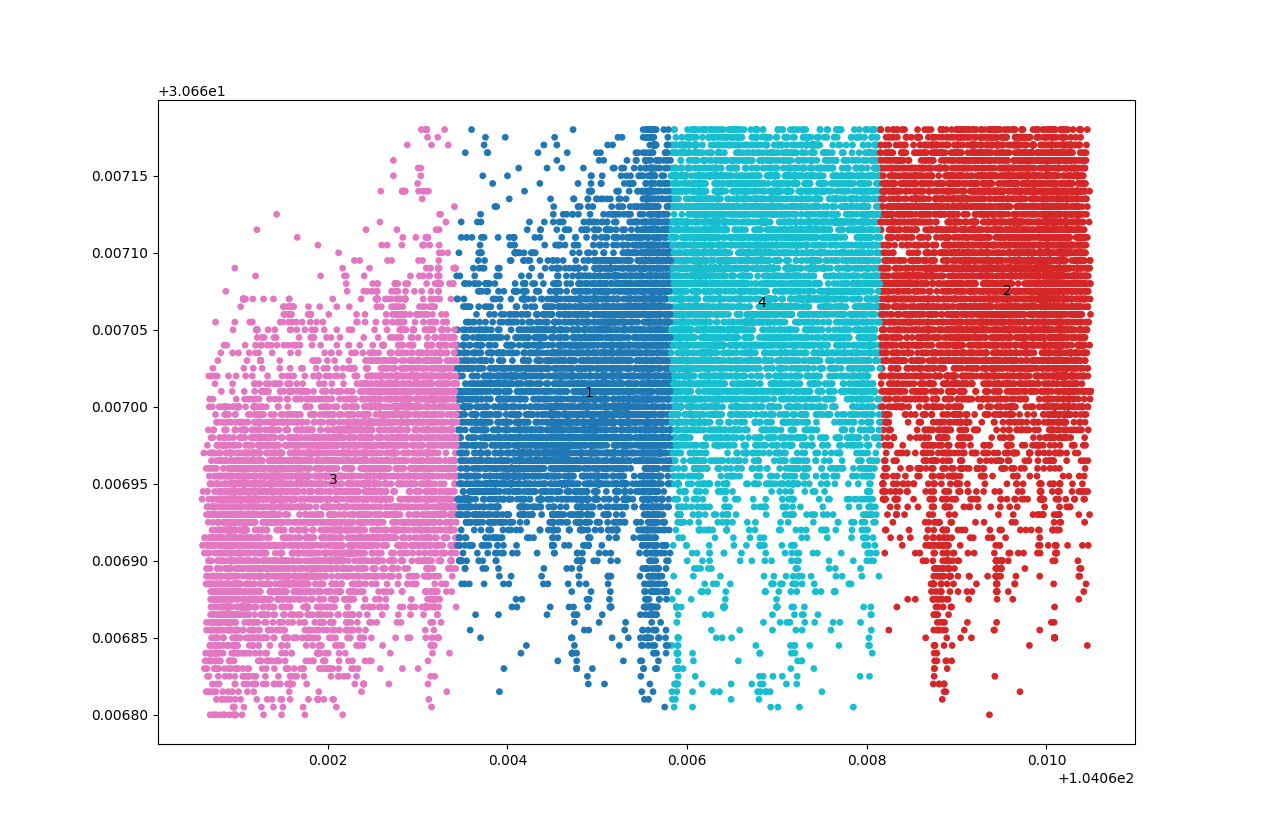
\includegraphics[width=\textwidth]{images/20000辆车kmeans.png}
  \caption{20000 Taxis K-Means}
  \label{fig: 20000}
\end{figure}

Thus, we end up with using the data of 20000 taxis, including 36940 GPS points and 36939 midpoints.
And we get a really nice result of segments.

\subsection{Result}
Here we get 4 segments, partitioned by longitude.

\begin{enumerate}
  \item \textrm{[104.06060, 104.06346]}
  \item \textrm{[104.06347, 104.06580]}
  \item \textrm{[104.06581, 104.06814]}
  \item \textrm{[104.06815, 104.07049]}
\end{enumerate}

And their speeds are $2.92534\times10^{-5}, 2.96561\times10^{-5}, 3.61342\times10^{-5}, 1.63441\times10^{-5}$,
which meets our expectation of the distribution of speed.

In conclusion, the algorithm we proposed for computing \textit{Supersegment} is practical.

% \clearpage
% \phantomsection
% \addcontentsline{toc}{section}{References}
% \bibliographystyle{ieeetr}
% \bibliography{references}

\end{document}